The $2\Delta NLL$ (two times of difference in the negative of log likelihood) 
as a function of NPs is computed using the Command (\ref{cmd:deltaNLL}).
The plots showing the variation of $2\Delta NLL$ for different values of NPs 
are shown in Figure~\ref{fig:nuisScan1}--\ref{fig:nuisScan13}. From these figures, 
one can see that $2\Delta NLL$ is symmetric for most of the parameters. However, 
the $2\Delta NLL$ is a bit constrained for those NPs which are profiled as 
"shape" in the data cards such as $hDamp\_tt$, $scaleRF\_tt$. Also, the $2\Delta 
NLL$ is asymmetric for few NPs which correspond to far higher and far lower bins 
of \mjj distribution (where the number of events is very small) such as 
$prop\_binch1\_bin29$, $prop\_binch1\_bin28$, $prop\_binch1\_bin3$ etc. Please 
note that the bin29 correspond to $30\times 5 + 20 = 170$ GeV of \mjj, 
because the binning in autoMCStats starts from 0 and the bin width is 5 GeV and 
there is a $20 \geq \mjj \geq 170$ GeV cut.

\newpage
\begin{figure}
    \centering  
    {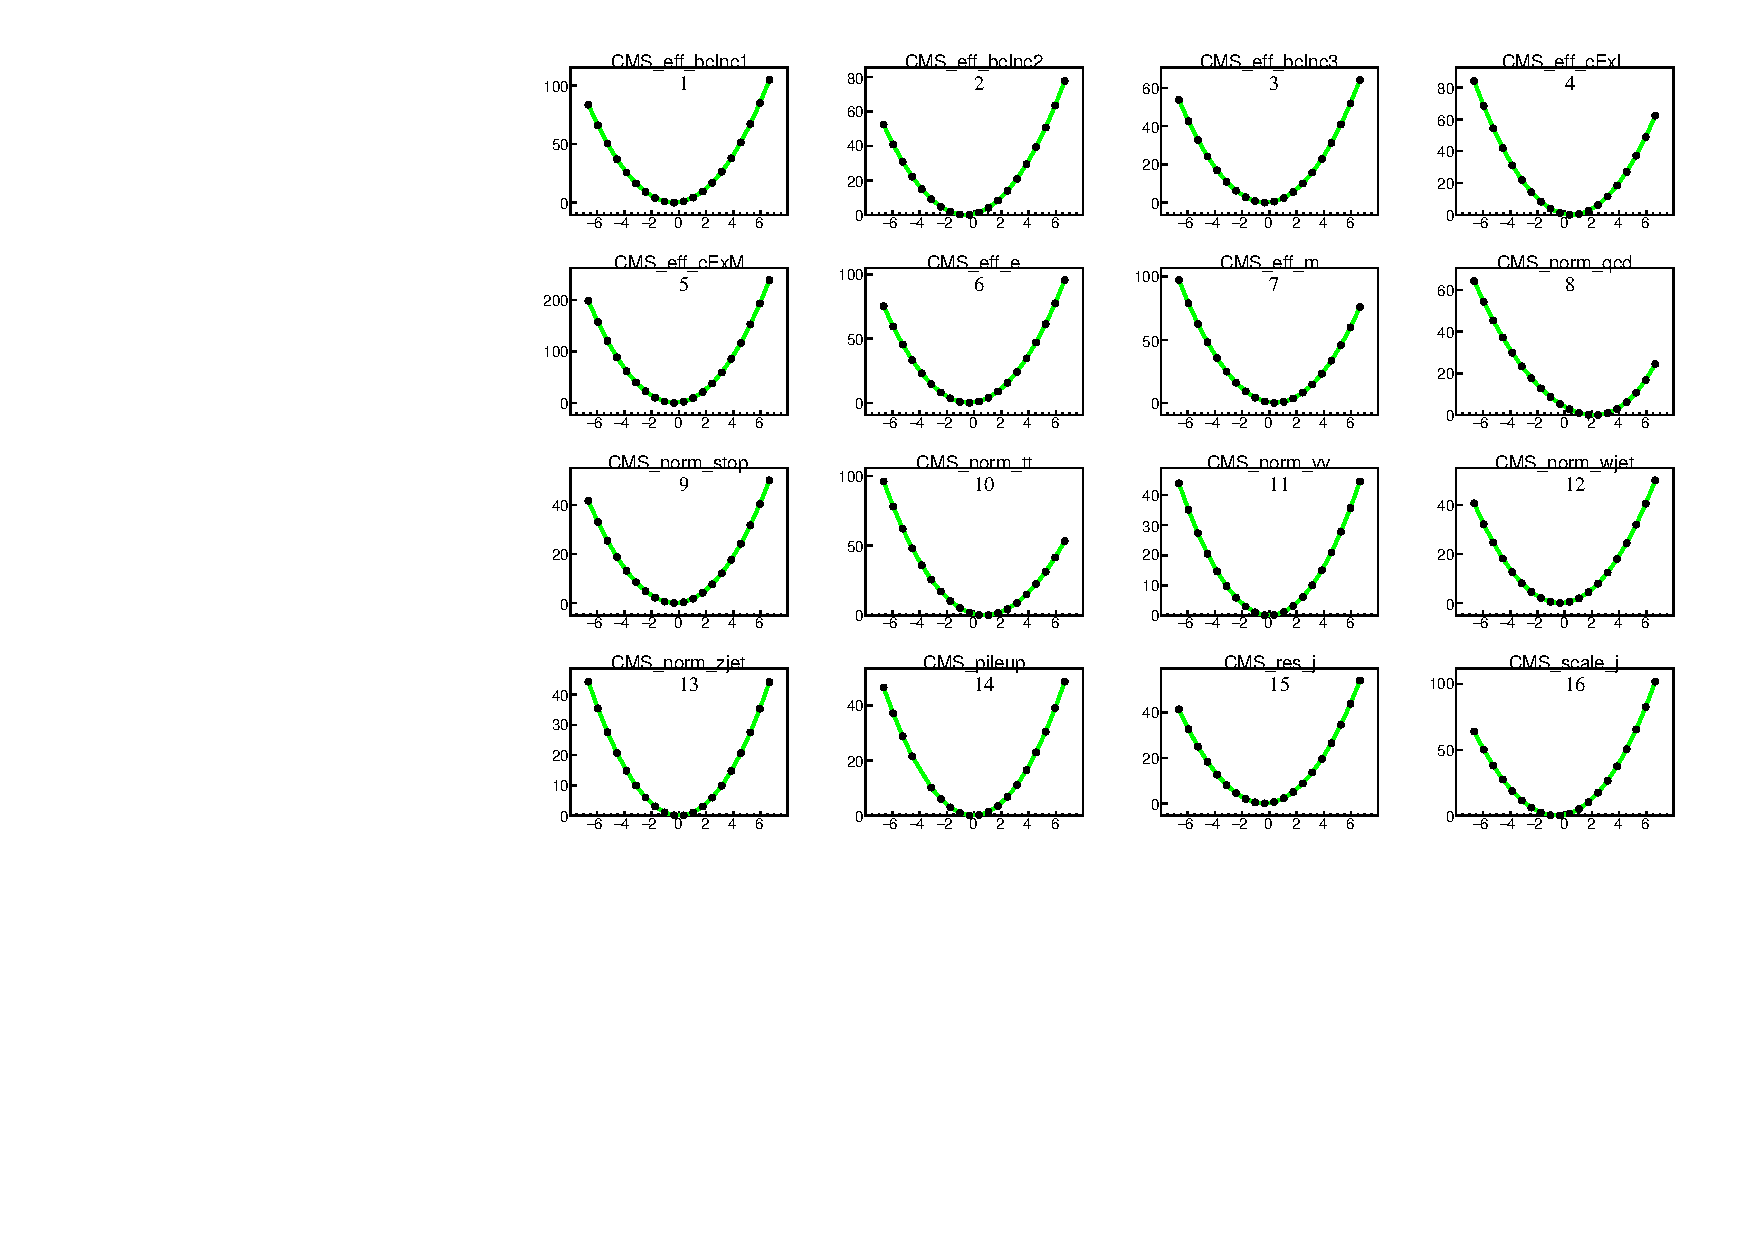
\includegraphics[width=1.0\linewidth]{Image/MLFit/ScanNuis/scanNuis1.pdf}}
    \caption{  $2\Delta NLL$ vs nuisance parameters. Contd ...}
    \label{fig:nuisScan1}
\end{figure}


\begin{figure}
    \centering  
    {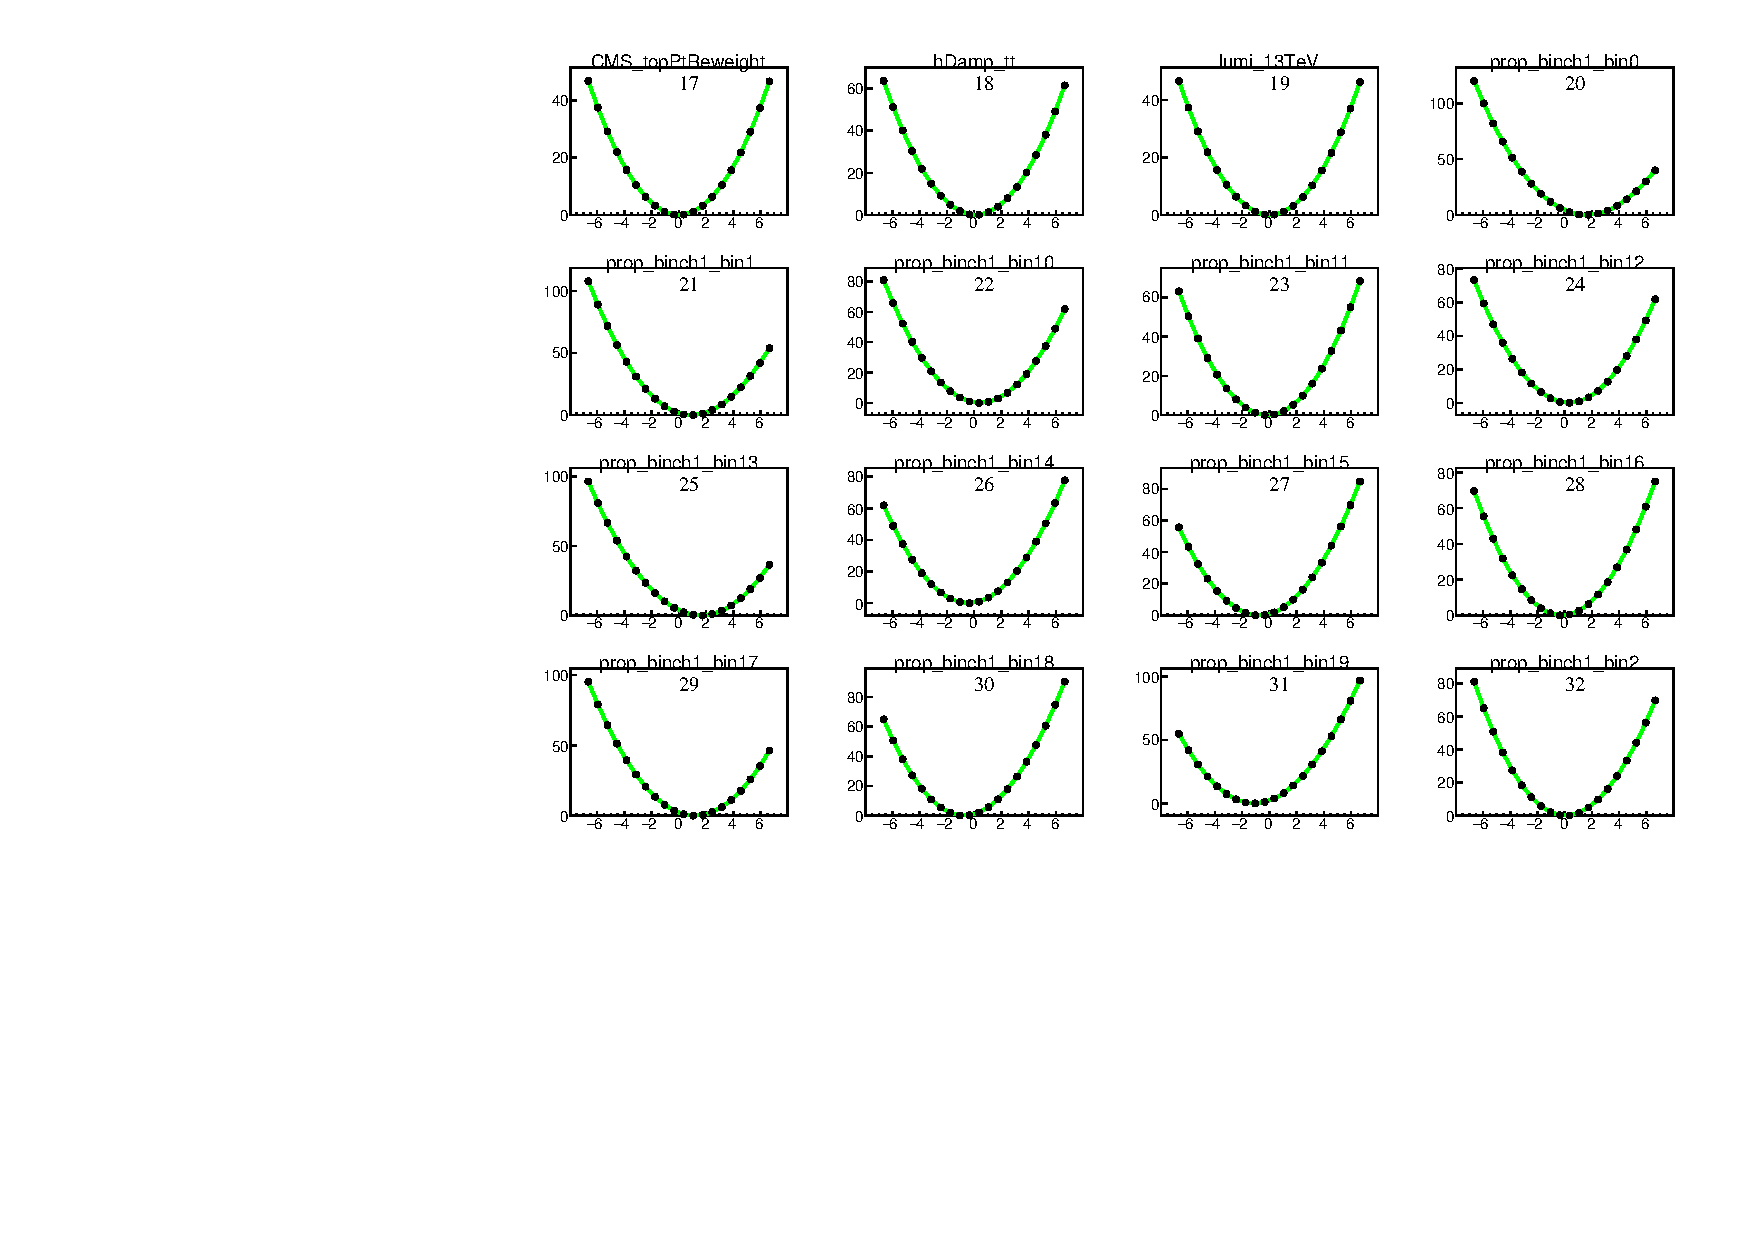
\includegraphics[width=1.0\linewidth]{Image/MLFit/ScanNuis/scanNuis2.pdf}}
    \caption{  $2\Delta NLL$ vs nuisance parameters. Contd ...}
    \label{fig:nuisScan2}
\end{figure}
\begin{figure}
    \centering  
    {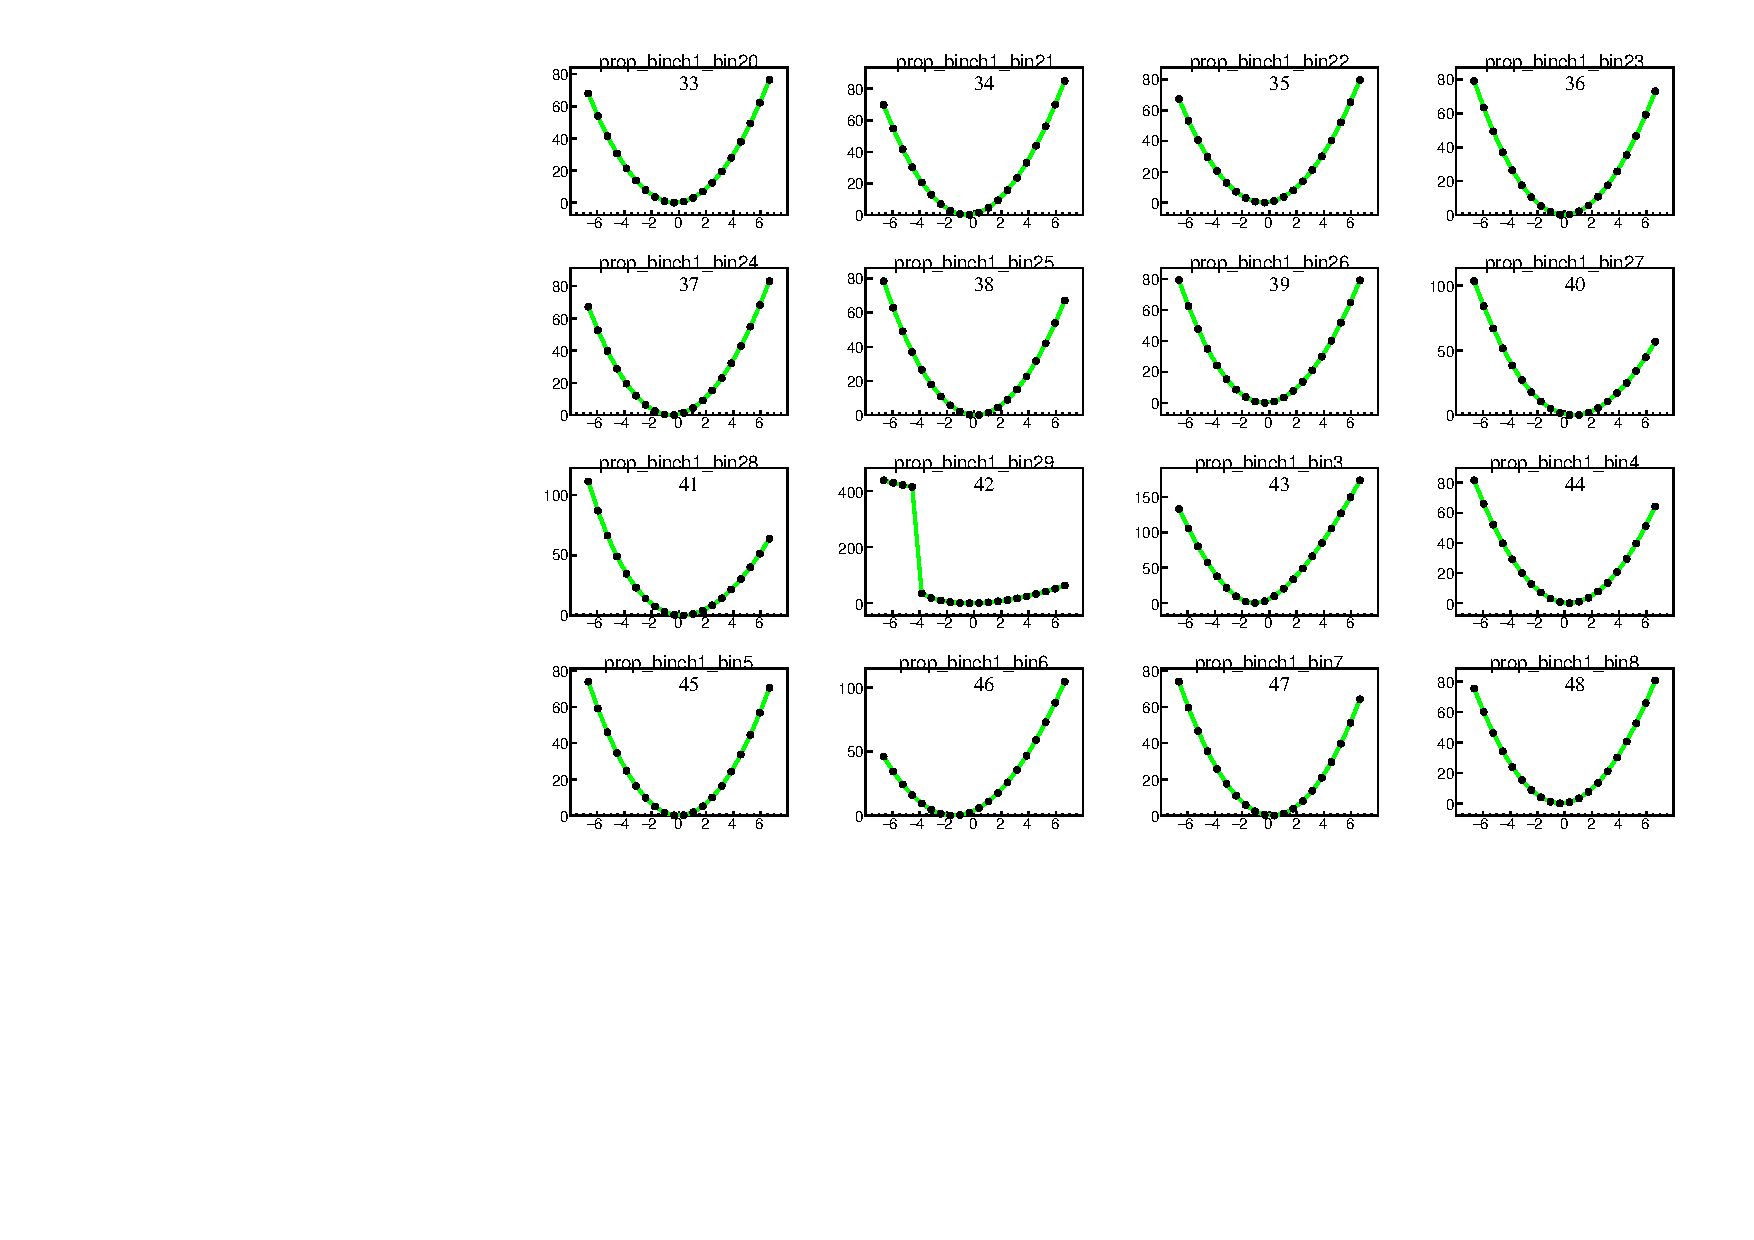
\includegraphics[width=1.0\linewidth]{Image/MLFit/ScanNuis/scanNuis3.pdf}}
    \caption{  $2\Delta NLL$ vs nuisance parameters. Contd ...}
    \label{fig:nuisScan3}
\end{figure}


\begin{figure}
    \centering  
    {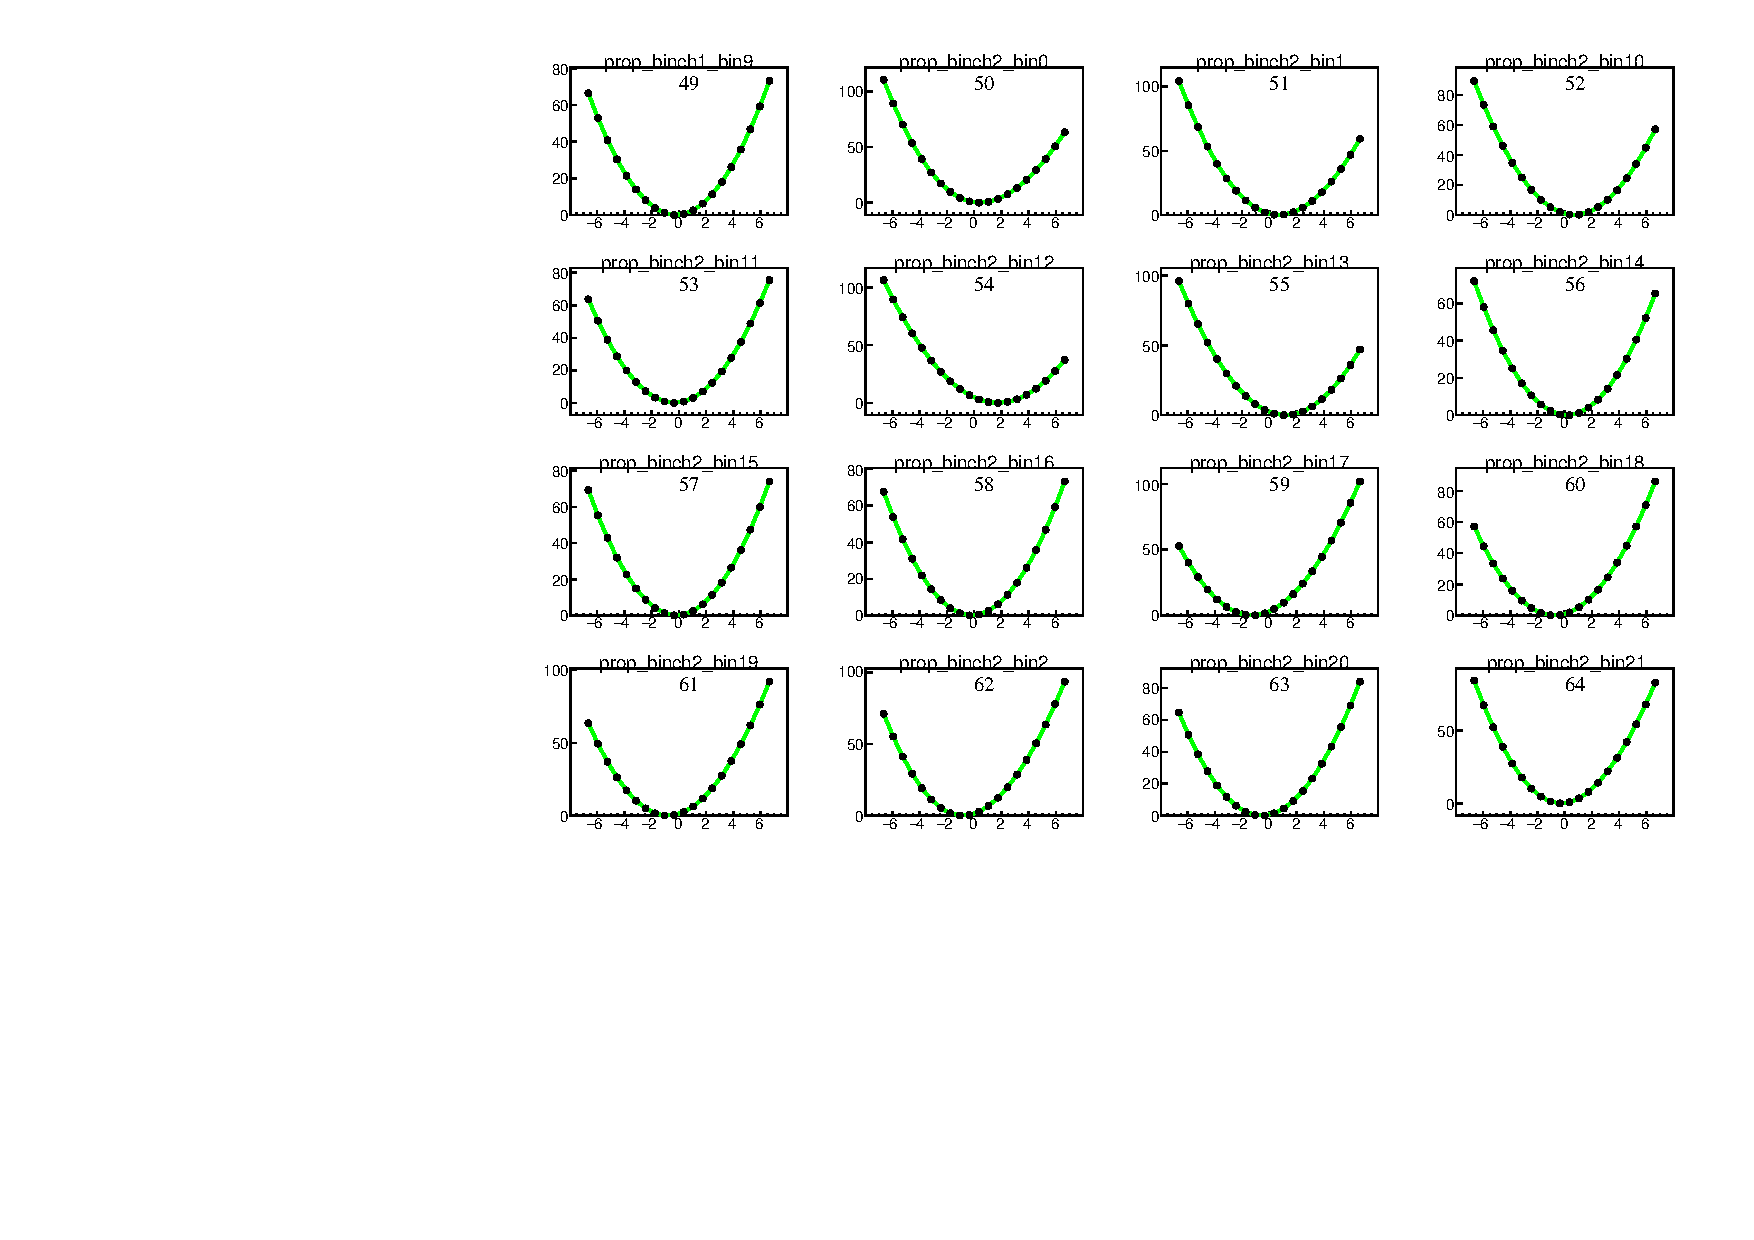
\includegraphics[width=1.0\linewidth]{Image/MLFit/ScanNuis/scanNuis4.pdf}}
    \caption{  $2\Delta NLL$ vs nuisance parameters. Contd ...}
    \label{fig:nuisScan4}
\end{figure}
\begin{figure}
    \centering  
    {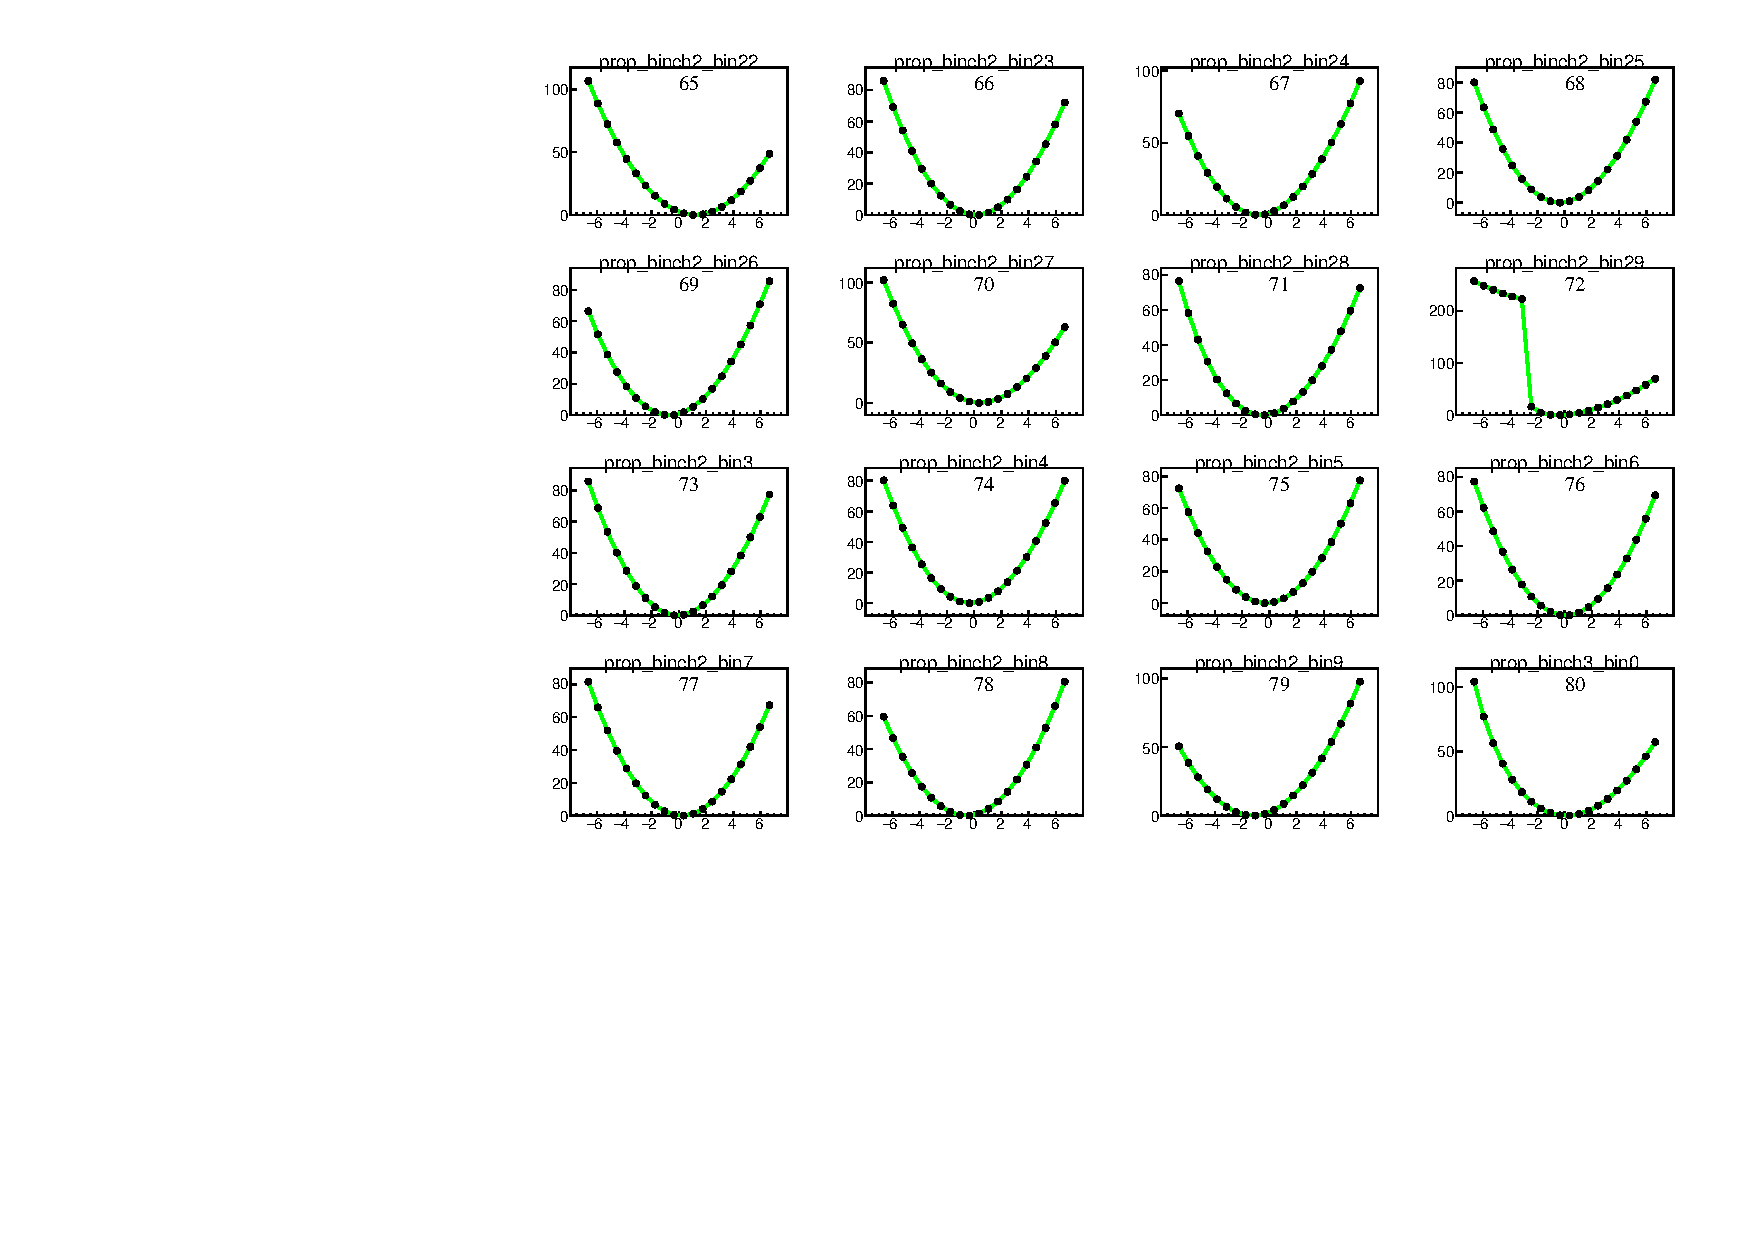
\includegraphics[width=1.0\linewidth]{Image/MLFit/ScanNuis/scanNuis5.pdf}}
    \caption{  $2\Delta NLL$ vs nuisance parameters. Contd ...}
    \label{fig:nuisScan5}
\end{figure}


\begin{figure}
    \centering  
    {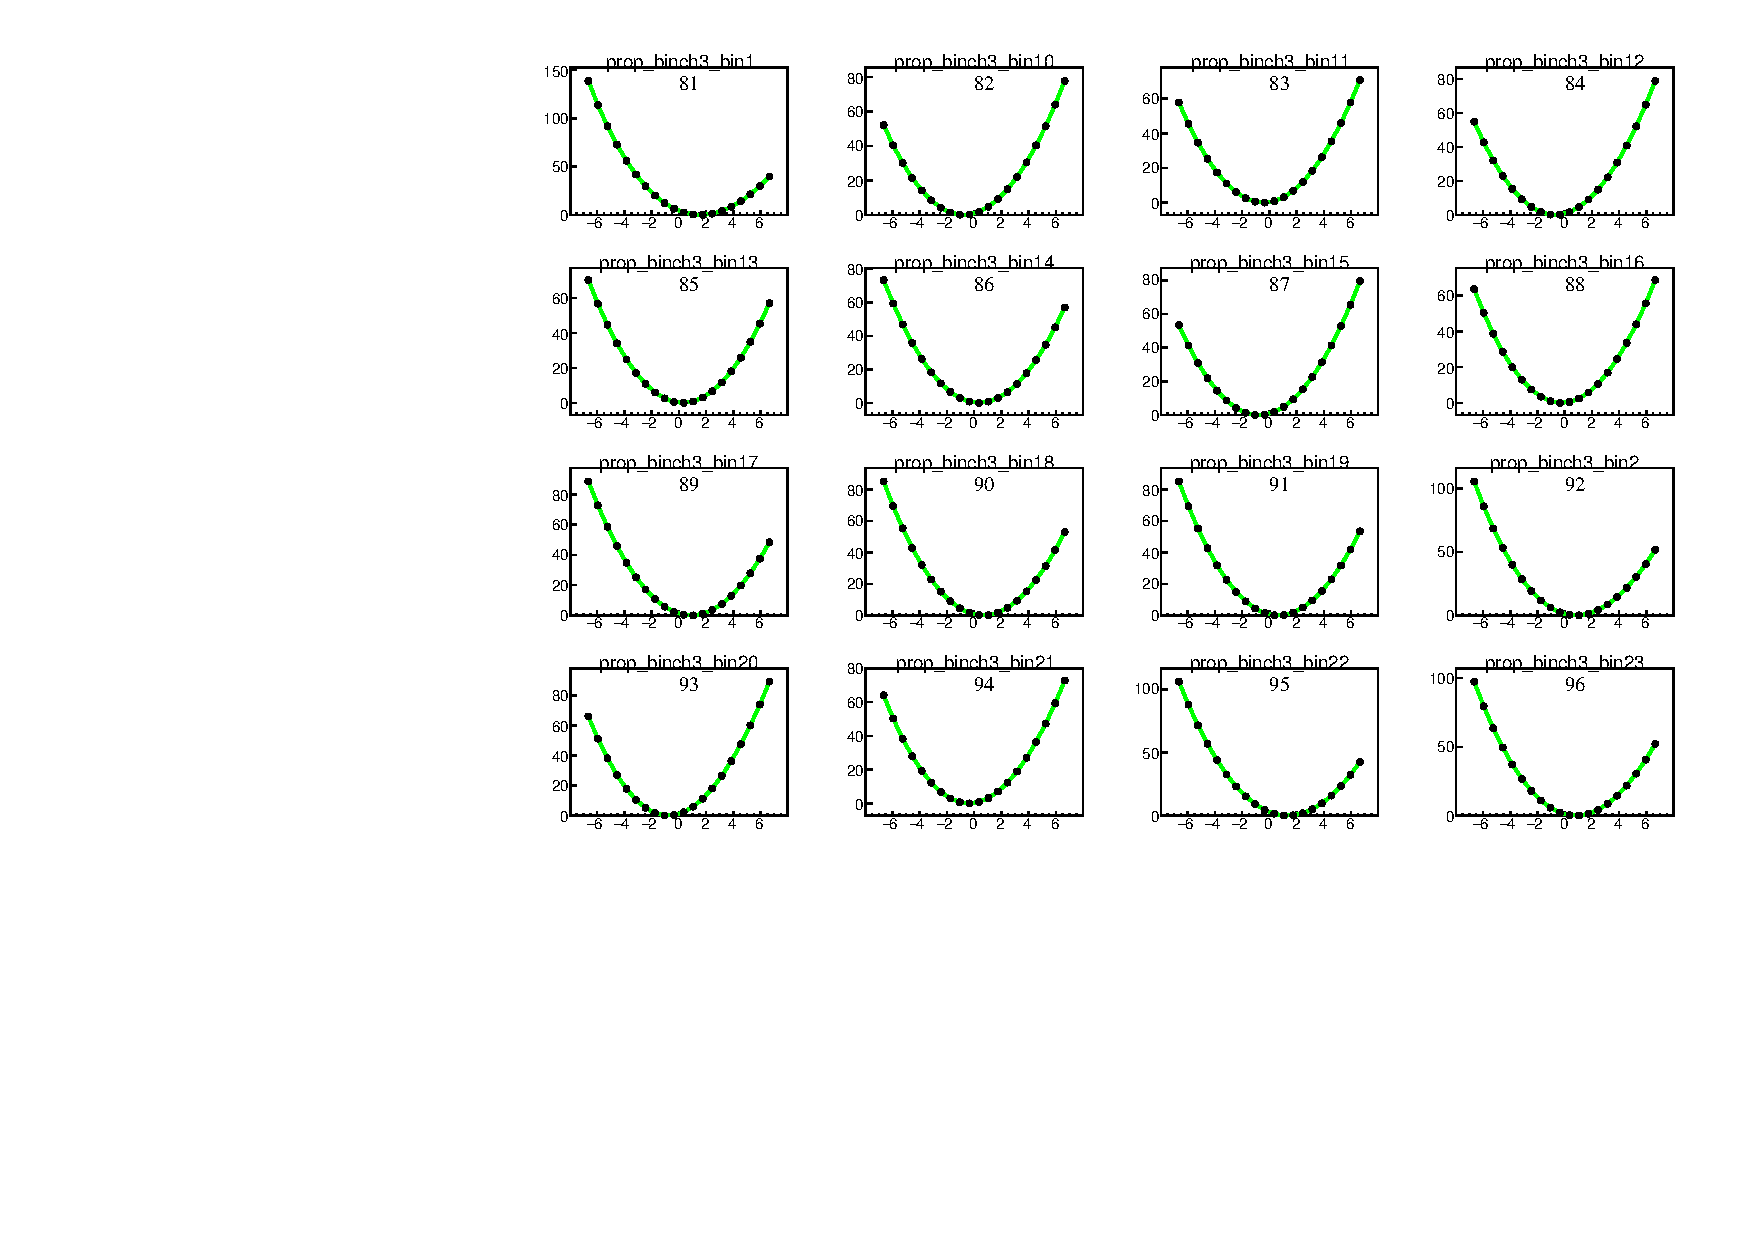
\includegraphics[width=1.0\linewidth]{Image/MLFit/ScanNuis/scanNuis6.pdf}}
    \caption{  $2\Delta NLL$ vs nuisance parameters. Contd ...}
    \label{fig:nuisScan6}
\end{figure}

\begin{figure}
    \centering  
    {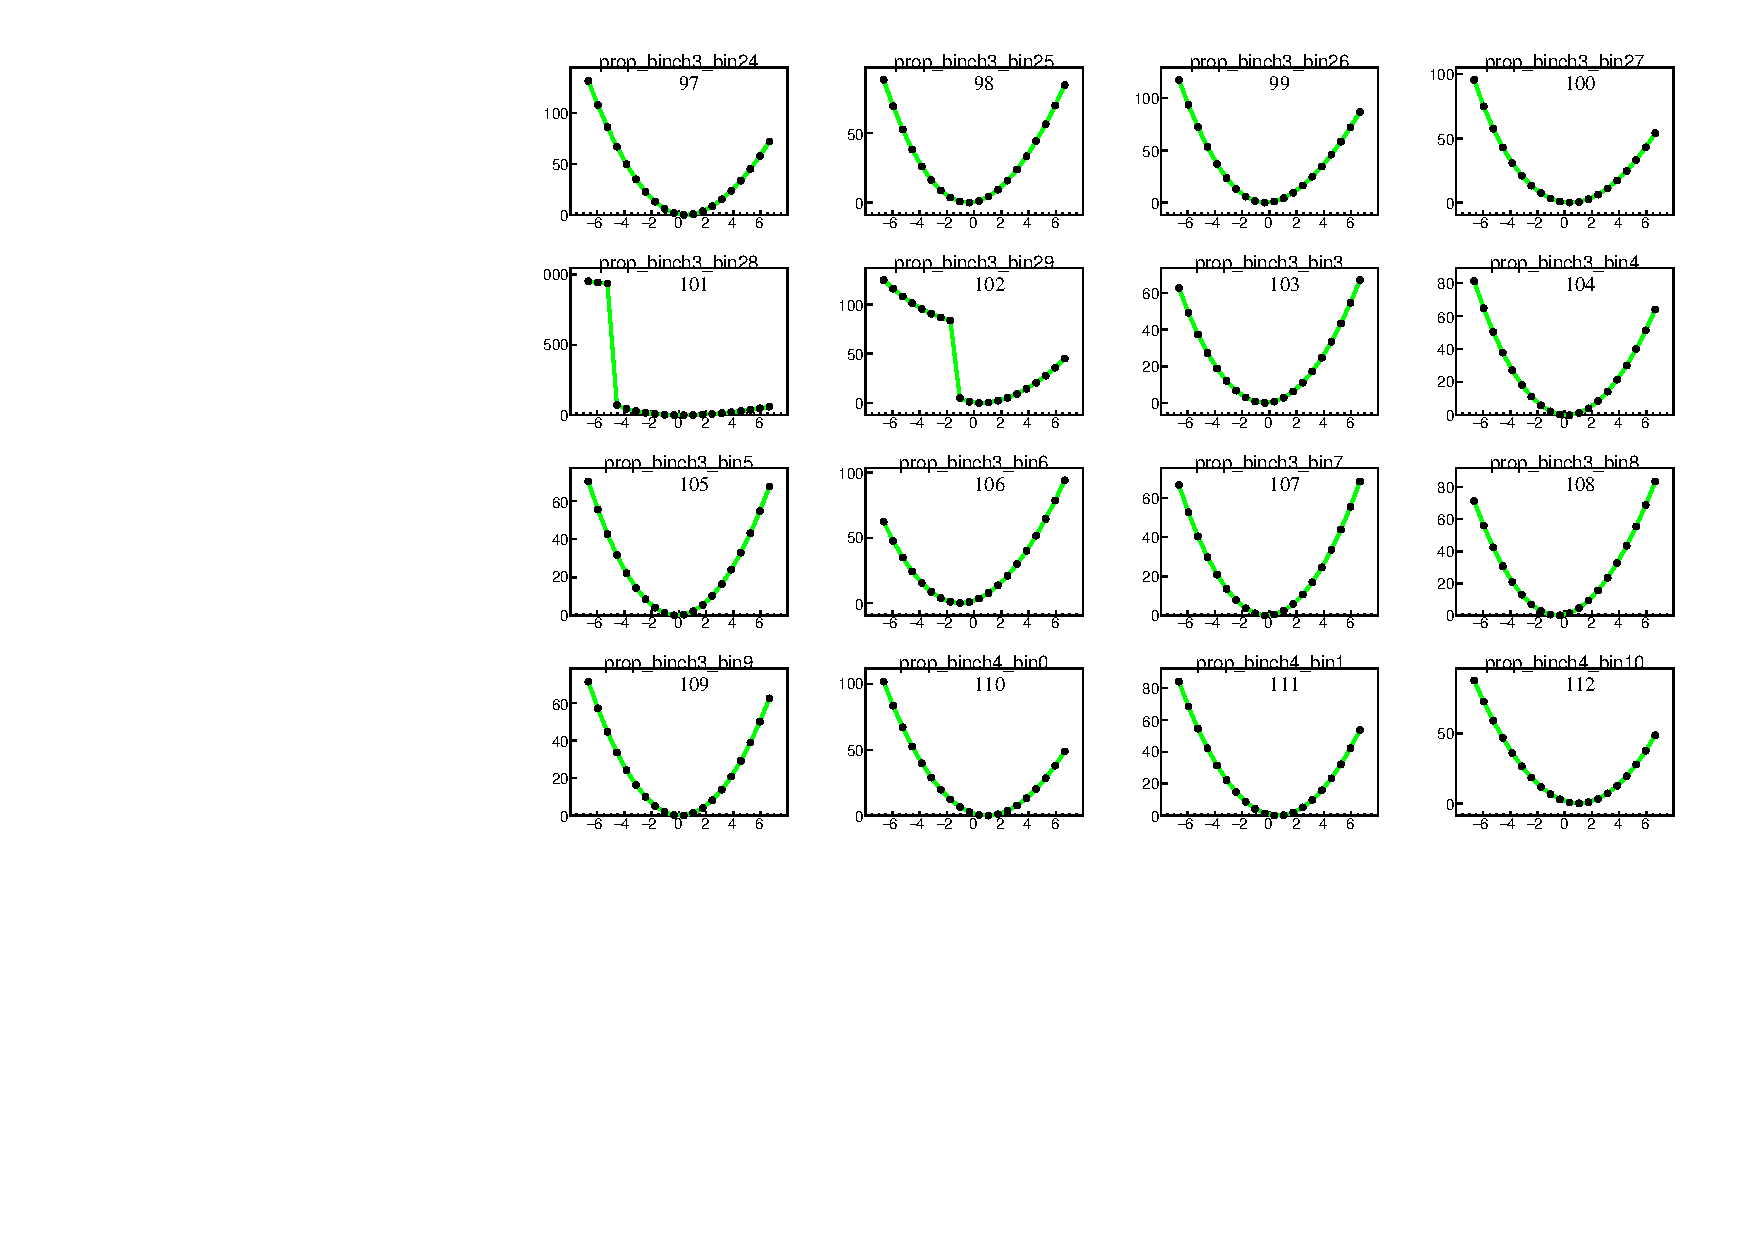
\includegraphics[width=1.0\linewidth]{Image/MLFit/ScanNuis/scanNuis7.pdf}}
    \caption{  $2\Delta NLL$ vs nuisance parameters. Contd ...}
    \label{fig:nuisScan7}
\end{figure}
\begin{figure}
    \centering  
    {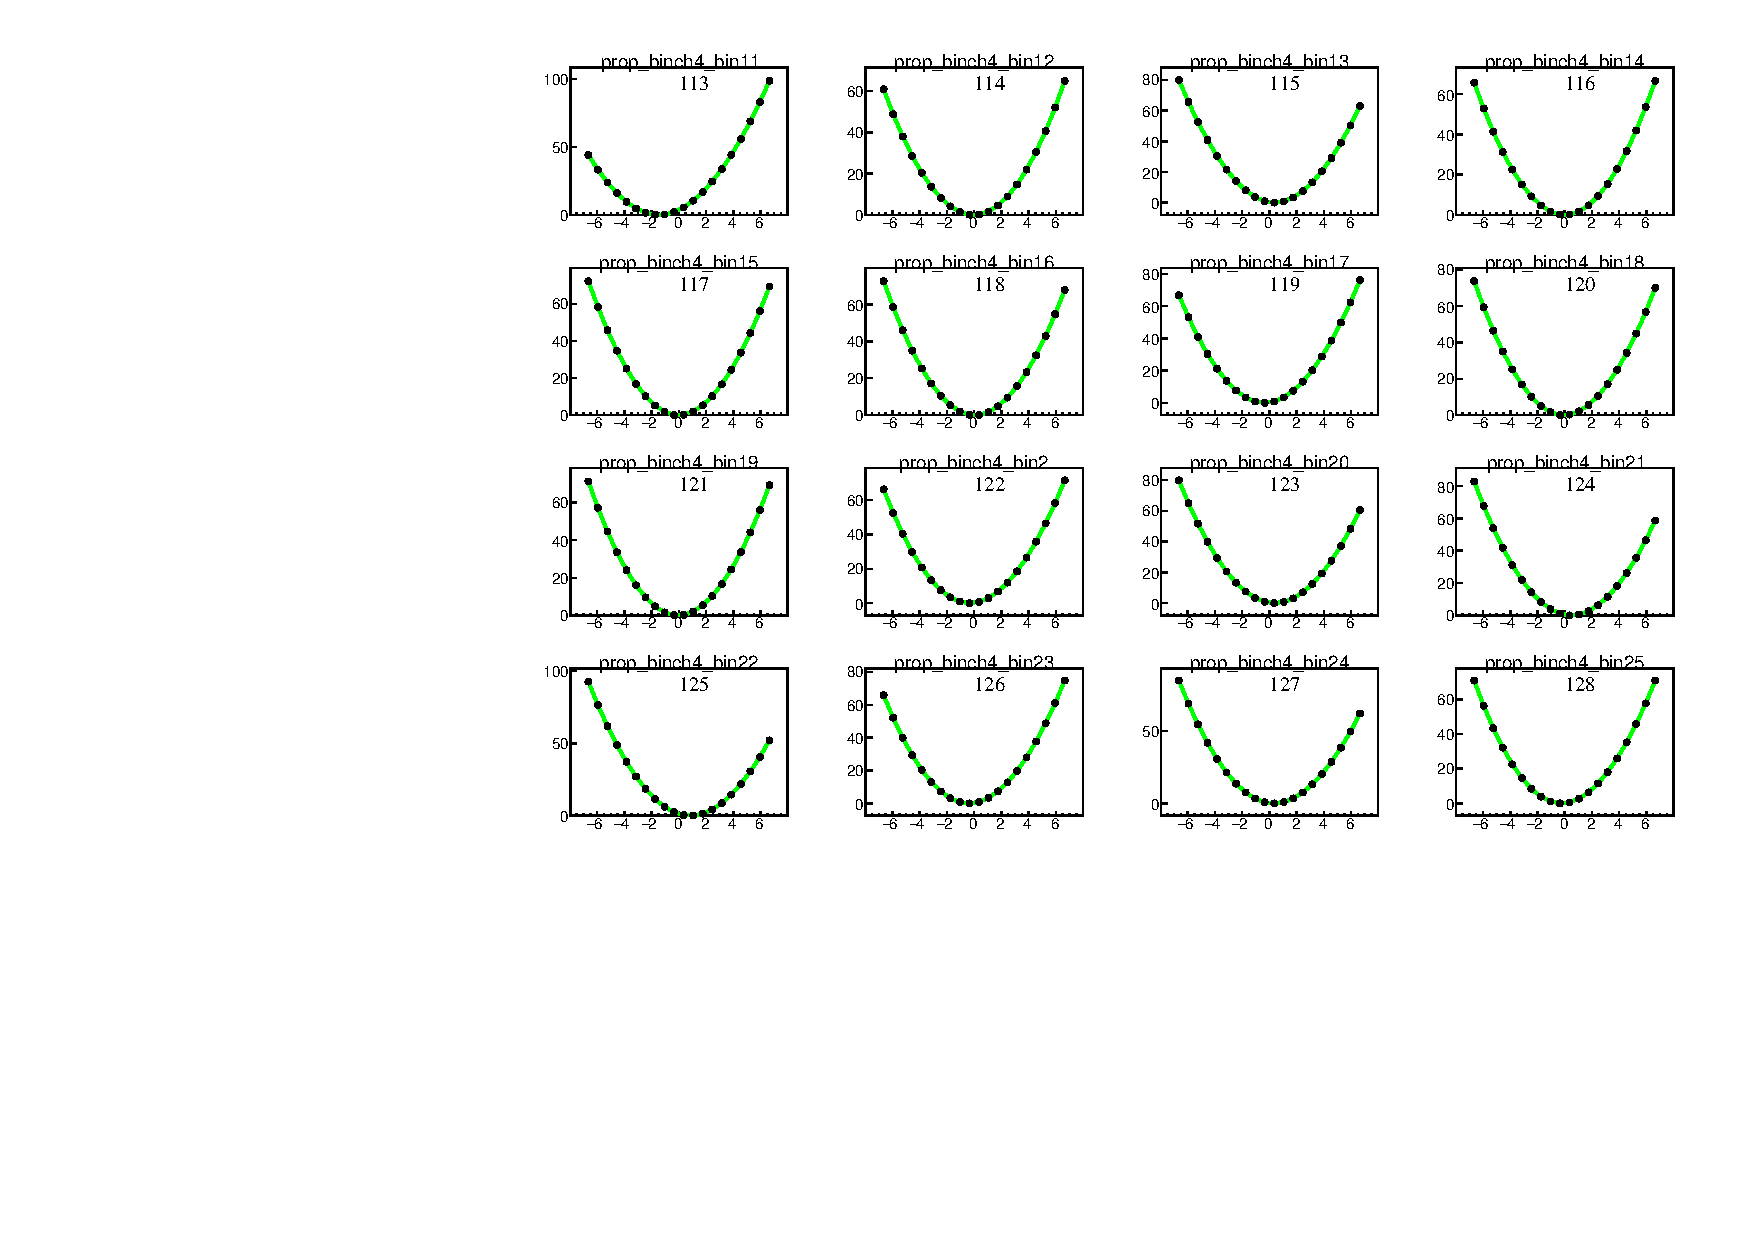
\includegraphics[width=1.0\linewidth]{Image/MLFit/ScanNuis/scanNuis8.pdf}}
    \caption{  $2\Delta NLL$ vs nuisance parameters. Contd ...}
    \label{fig:nuisScan8}
\end{figure}
\begin{figure}
    \centering  
    {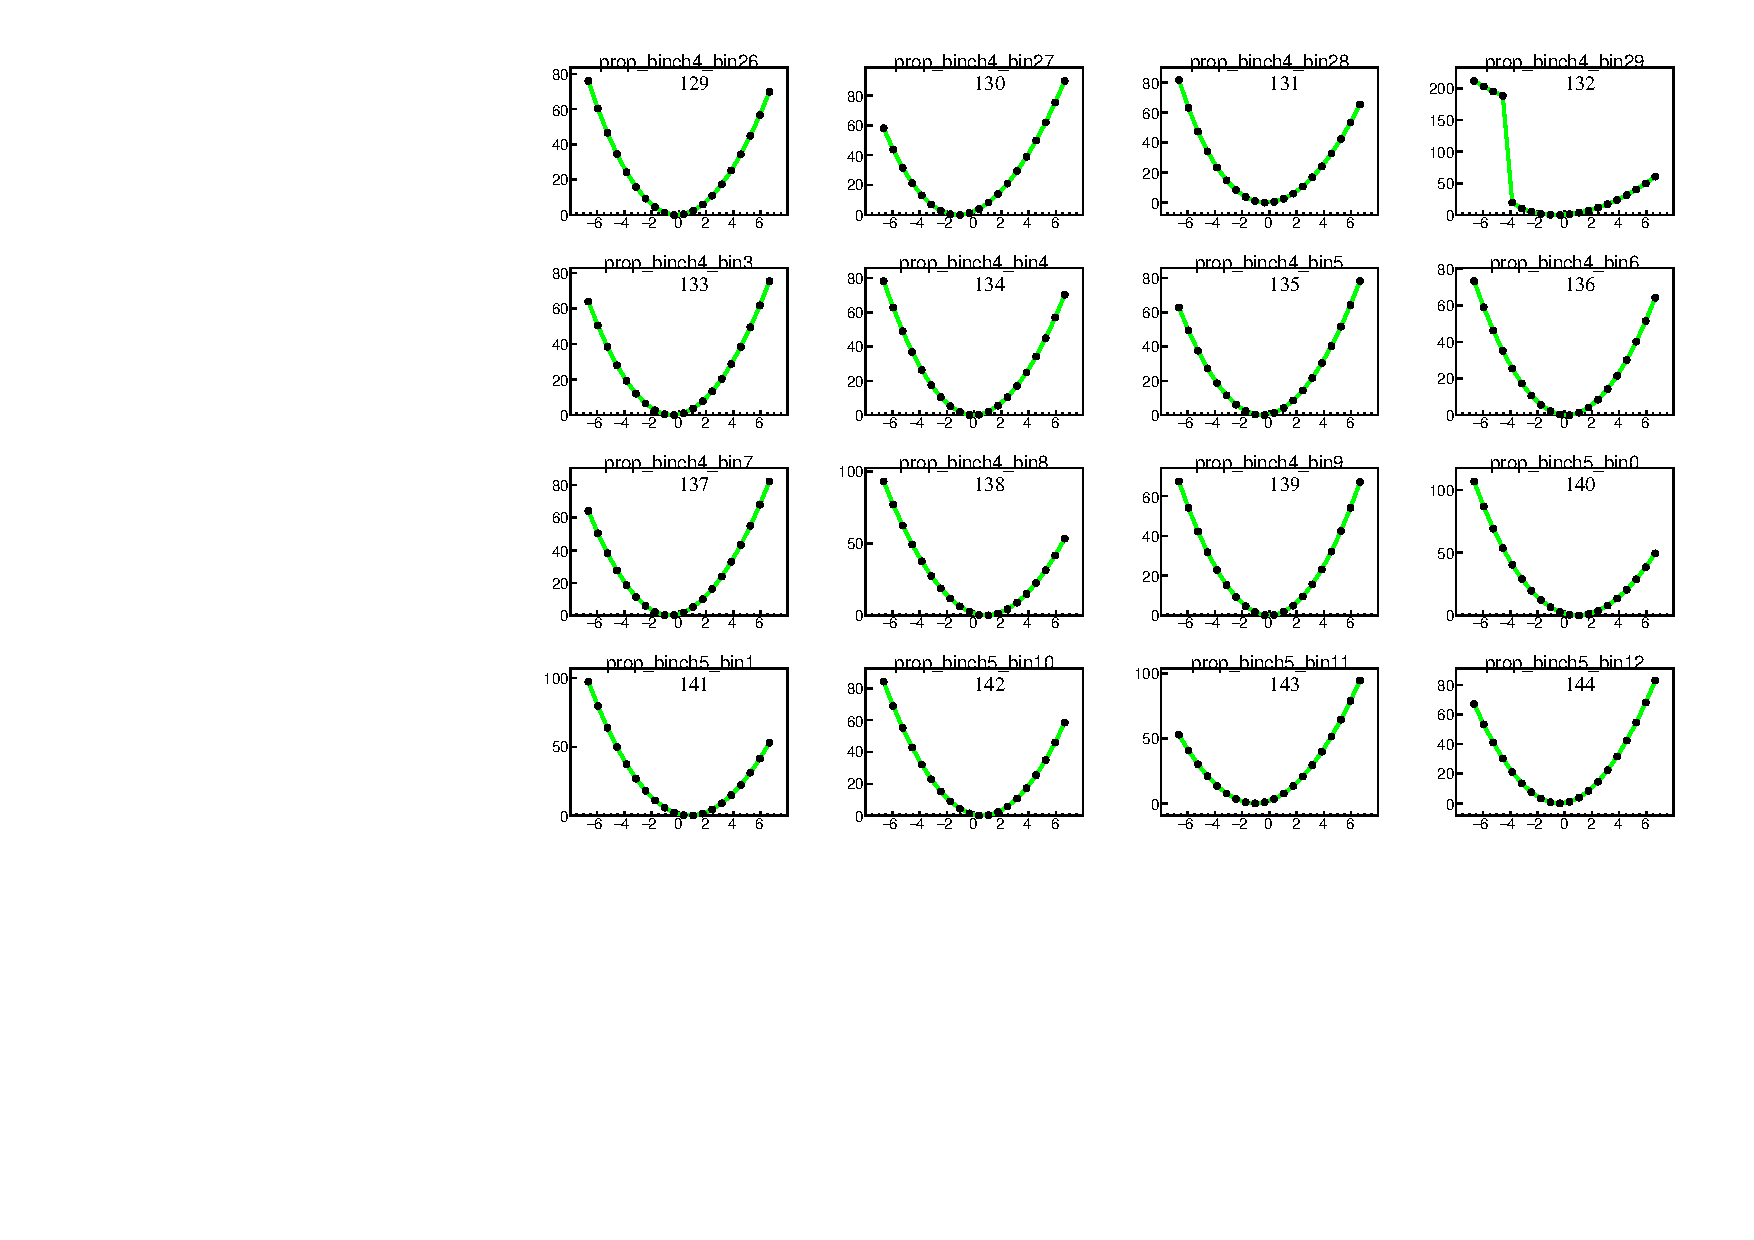
\includegraphics[width=1.0\linewidth]{Image/MLFit/ScanNuis/scanNuis9.pdf}}
    \caption{  $2\Delta NLL$ vs nuisance parameters. Contd ...}
    \label{fig:nuisScan9}
\end{figure}
\begin{figure}
    \centering  
    {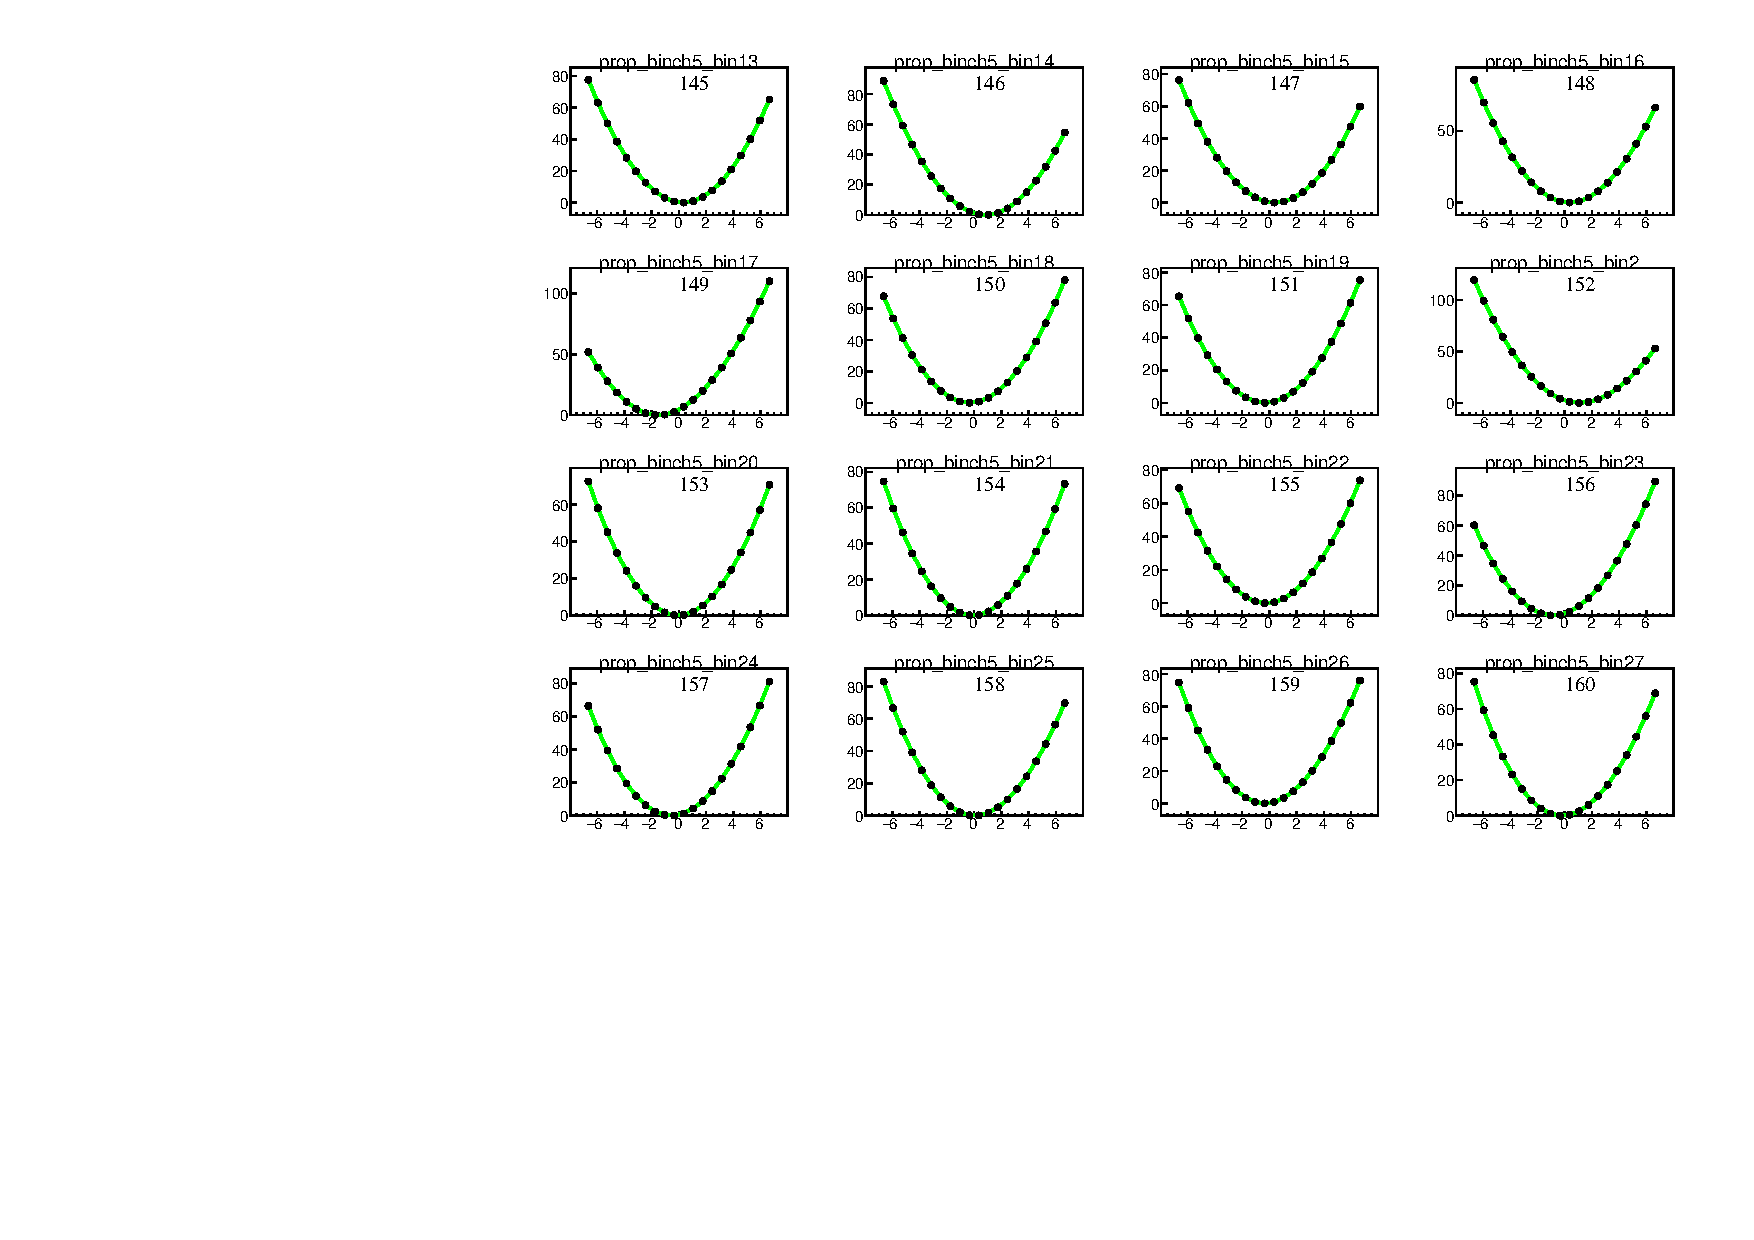
\includegraphics[width=1.0\linewidth]{Image/MLFit/ScanNuis/scanNuis10.pdf}}
    \caption{  $2\Delta NLL$ vs nuisance parameters. Contd ...}
    \label{fig:nuisScan10}
\end{figure}
\begin{figure}
    \centering  
    {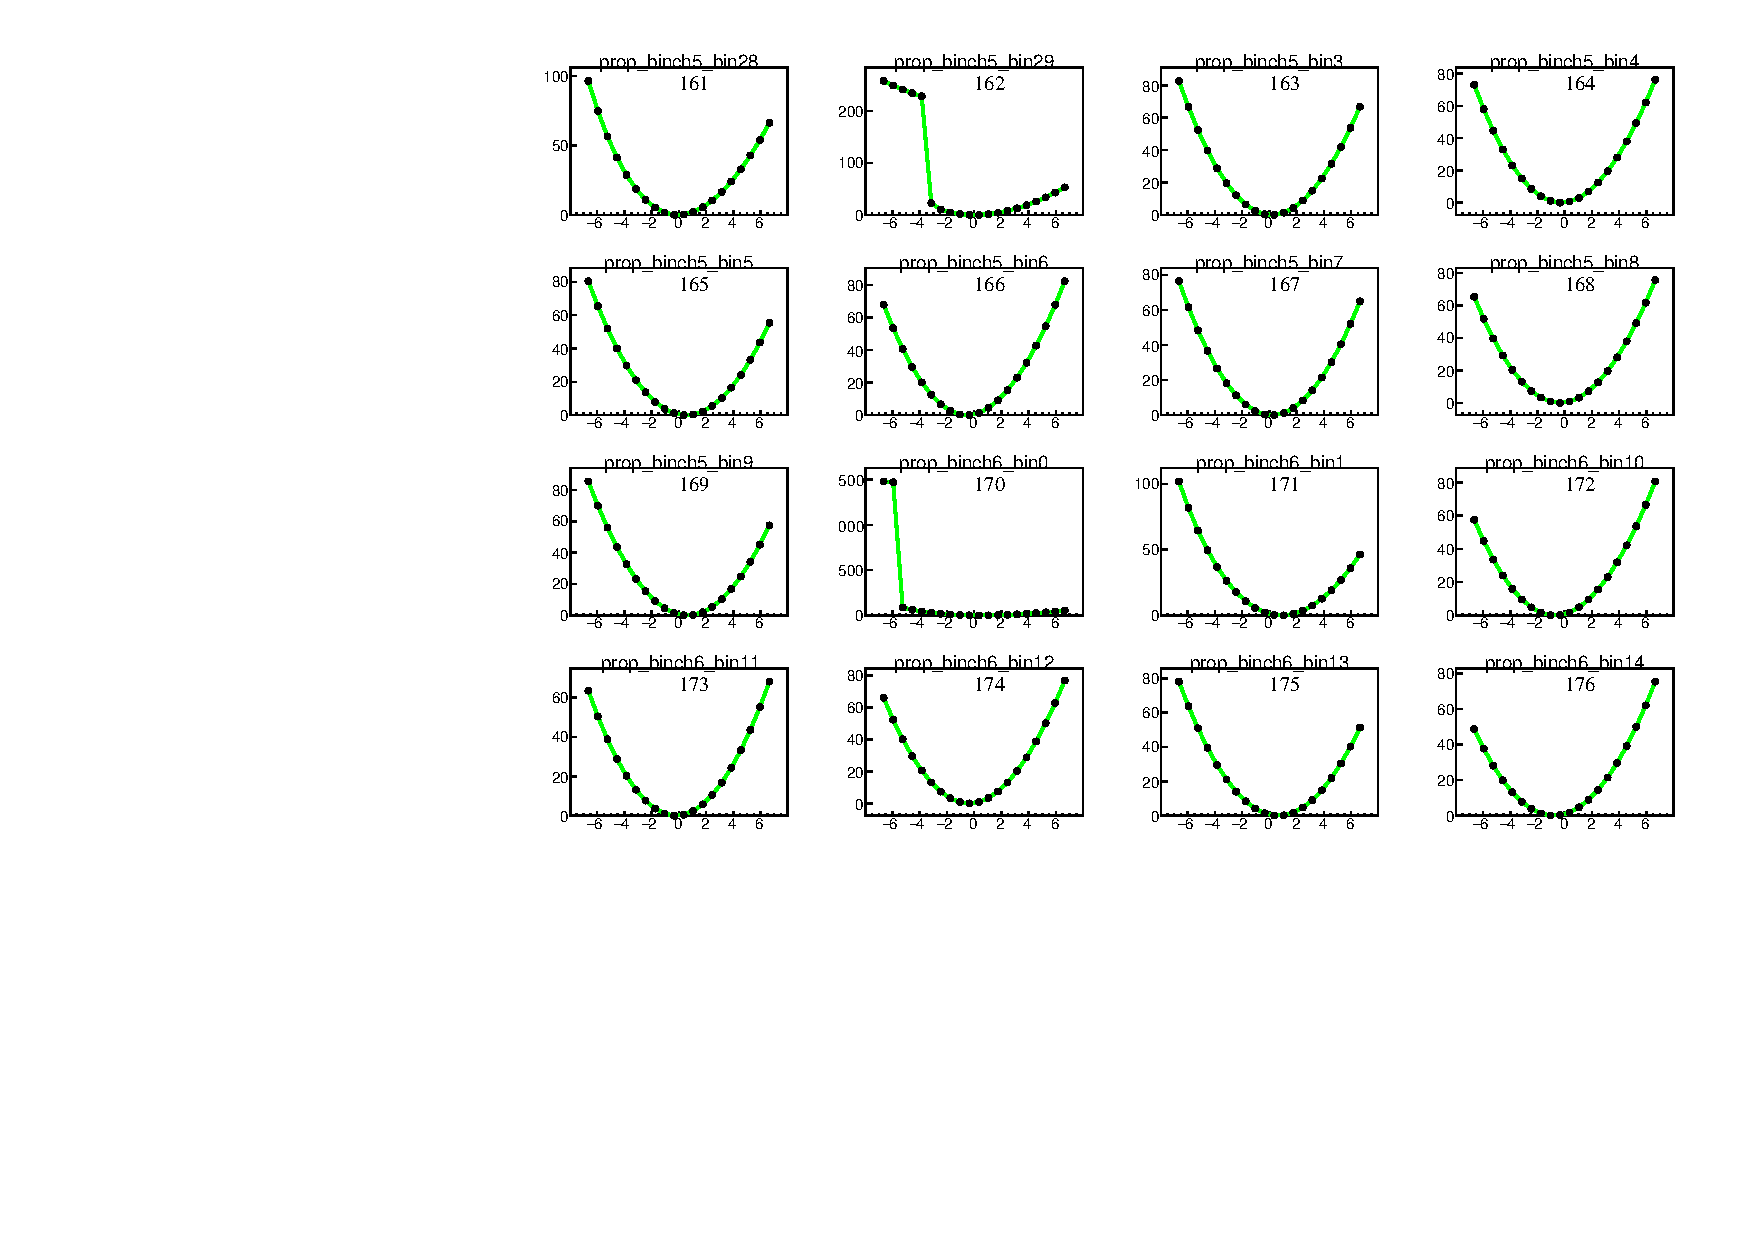
\includegraphics[width=1.0\linewidth]{Image/MLFit/ScanNuis/scanNuis11.pdf}}
    \caption{  $2\Delta NLL$ vs nuisance parameters. Contd ...}
    \label{fig:nuisScan11}
\end{figure}
\begin{figure}
    \centering  
    {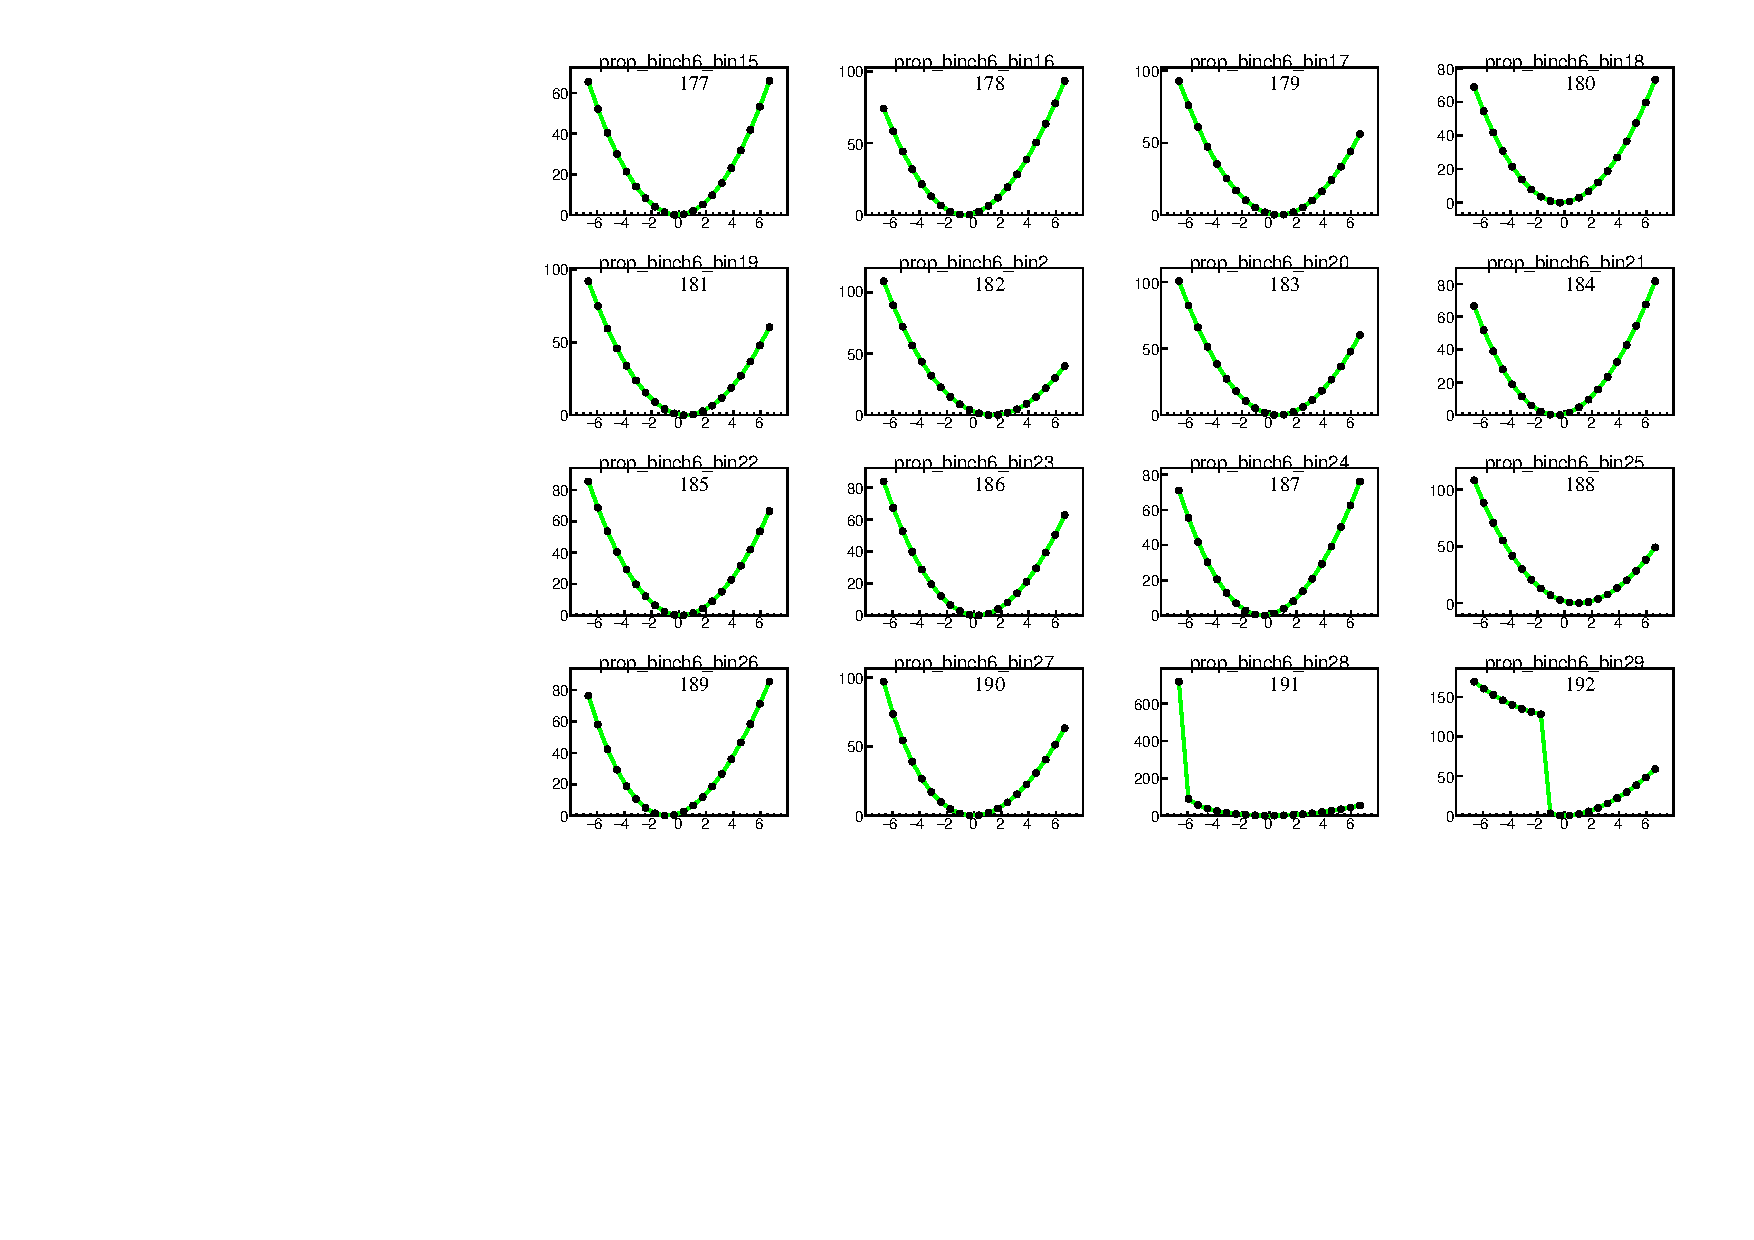
\includegraphics[width=1.0\linewidth]{Image/MLFit/ScanNuis/scanNuis12.pdf}}
    \caption{  $2\Delta NLL$ vs nuisance parameters. Contd ...}
    \label{fig:nuisScan12}
\end{figure}

\begin{figure}
    \centering  
    {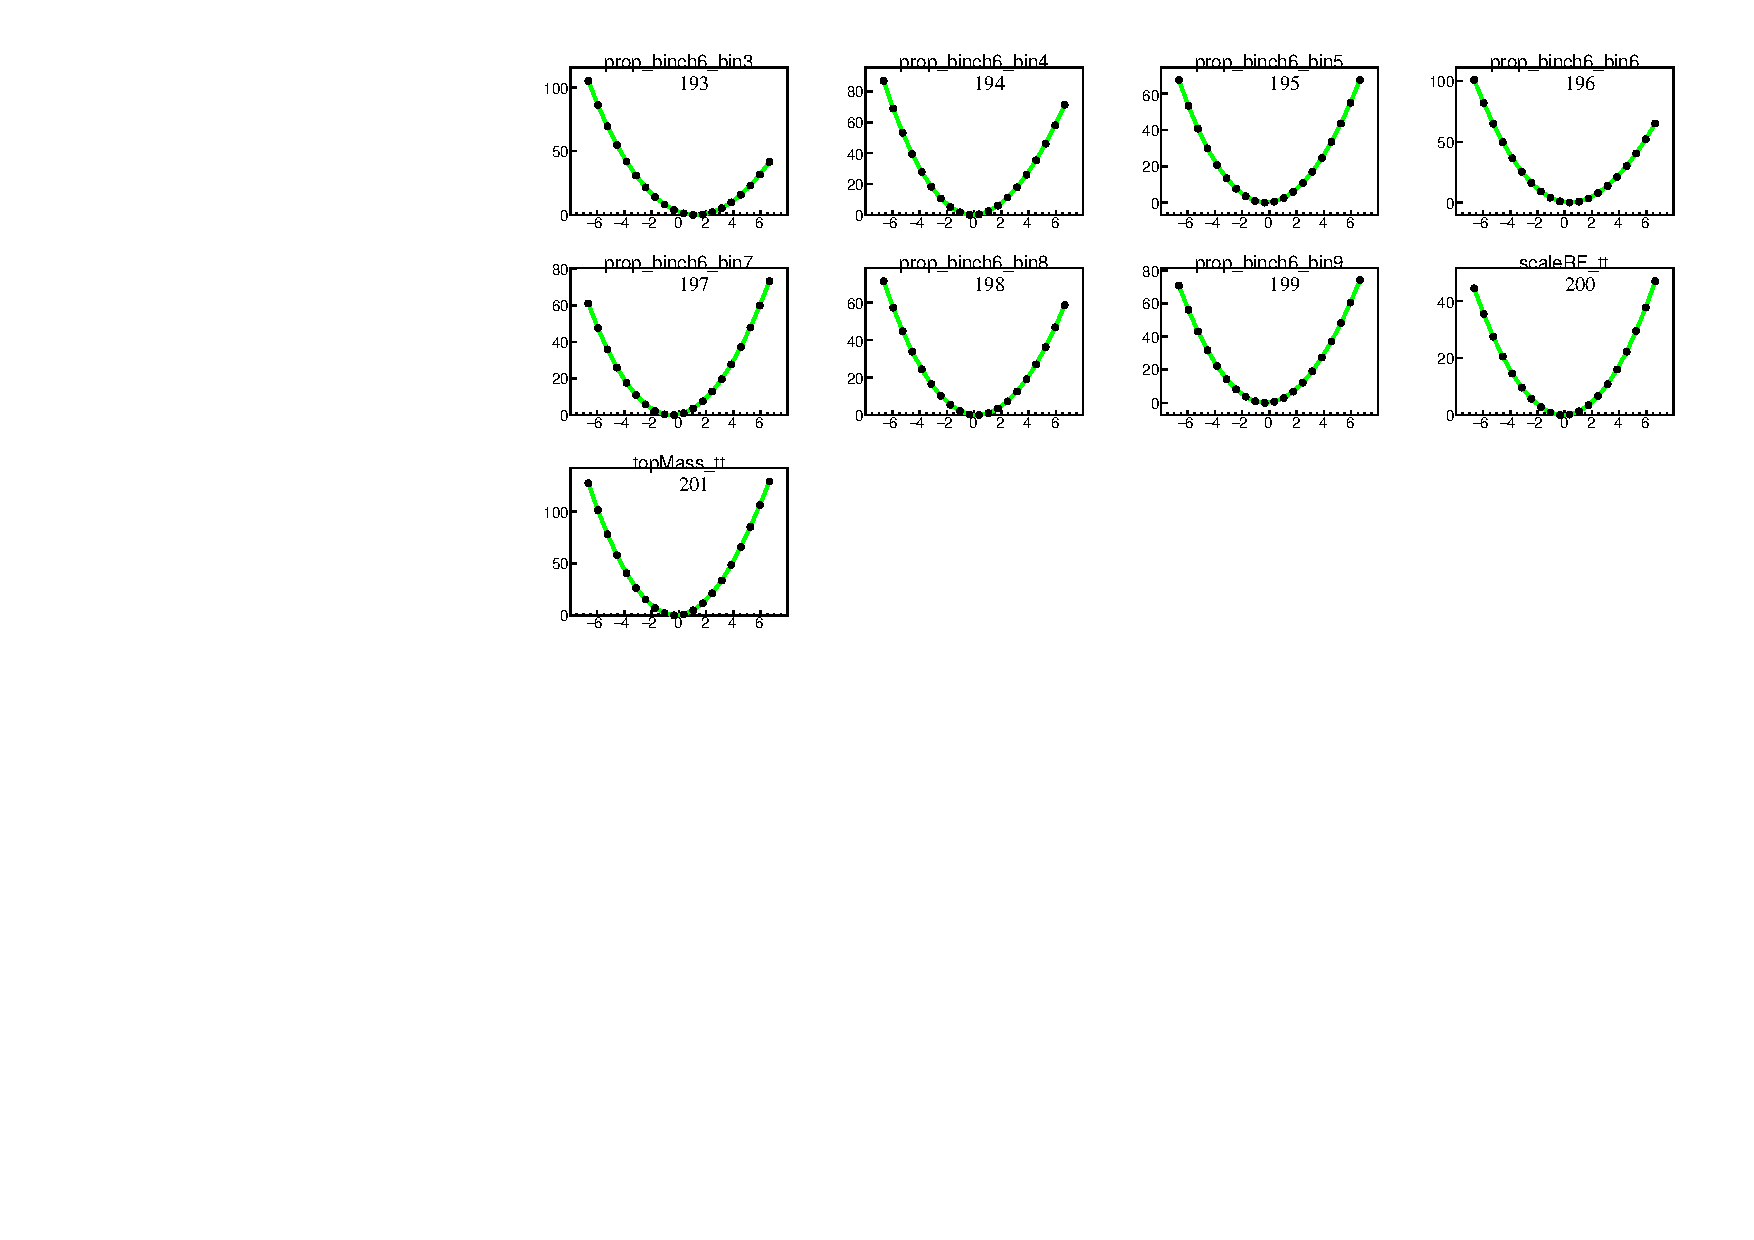
\includegraphics[width=1.0\linewidth]{Image/MLFit/ScanNuis/scanNuis13.pdf}}
    \caption{  $2\Delta NLL$ vs nuisance parameters.}
    \label{fig:nuisScan13}
\end{figure}

